% !TeX spellcheck = en_GB
\documentclass[11pt]{article}
\usepackage{graphicx}
\usepackage{listings}
\usepackage[T1]{fontenc}
\title{Machine Learning Project\\Task 3: Reinforcement Learning}
\author{Duy Nguyen Dinh \\ dinh@rhrk.uni-kl.de\and
	Minh Duc Duong\\ duong@rhrk.uni-kl.de\and
    }
\date{\today}
\begin{document}

\maketitle

\section{Tabular Reinforcement Learning}

\subsection{Introduction to reinforcement learning}
Reinforcement learning is a type of learning, which results actions based on certain situation with the goal to maximize a specific value (reward signal). In the beginning, the model does not know what to do to maximize the reward but it must try to find out by itself through trials and errors. Each time the model try to learn the situation can either have the same parameters or affected by actions from the past learning, which is mentioned as delayed reward.

One of the problem of reinforcement learning is Markov decision process. This problem requires evaluate the outcome and choosing actions base on different situation to maximize the reward signal. The learner is called agent, which also makes decisions throughout the learning process. In this case, making decisions (actions) is interacting with things outside the agent, which is called environment. Each time the agent performs an action, depend on the current state s and the environment, it will move to another state s' and yield a reward R, which we want to maximize the cumulative sum overtime. The reward is simply a rational number and is the result of reward function, which evaluate the actions and is the driving force of how the agent should behave. For example, we have a robot as an agent with the objective to escape a maze with the minimum amount of steps. Then the return function will yield a negative reward as we want the agent to take less steps as possible.

Now from a certain time t, we have a sequence of reward for the next steps as R\textsubscript{t+1},  R\textsubscript{t+2} ... R\textsubscript{T}, where T is the final step. The sum of these numbers is called return. Also at the time t, the agent has a certain state s and we want to evaluate how good this current state, which is how much potential reward can we gain from this state in the future (return). This is done by using value functions. Value functions defined by the ways the agent behaves, which is called policy. Policy is a mapping from states to probabilities of each possible actions. The notation is $\pi$(a$\vert$s), which is the probability the agent takes the action a if the current state is a. Thus the state-value function for Markov decision process can be defined as:

v\textsubscript{$\pi$}(s) = E\textsubscript{$\pi$}\big[ G\textsubscript{$t$}|S\textsubscript{t}=s \big] = E\textsubscript{$\pi$}\big[ $\sum_{k=0}^{\infty} \gamma^{k} R\textsubscript{t+k+1} | S\textsubscript{t}=s$ \big], for all s in S

where E\textsubscript{$\pi$}[$\bullet$] denoted as the expected value of random value given the time t and the policy $\pi$

We also define the value of taking action a in state s, denoted as q\textsubscript{$\pi$}(s$\vert$a).
This is action-value function for policy $\pi$

q\textsubscript{$\pi$}(s$\vert$a) = E\textsubscript{$\pi$}\big[ G\textsubscript{$t$}|S\textsubscript{t}=s,  A\textsubscript{t}=a \big] = E\textsubscript{$\pi$}\big[ $\sum_{k=0}^{\infty} \gamma^{k} R\textsubscript{t+k+1} | S\textsubscript{t}=s, A\textsubscript{t}=a $ \big]

For reinforcement learning, to maximize the return, we want to find the best policy at any given time. One policy can be better than the others. Its partial order can be defined using value function. If v\textsubscript{$\pi$}(s) >v\textsubscript{$\pi$'}(s) for all possible s, then $\pi$ is better than $\pi$'. Because there is one or more policies that are better than or equal to all others, these are optimal policy. If $\pi$ is an optimal policy, v\textsubscript{*}(s) is the optimal state-value function, which takes the maximum v\textsubscript{$\pi$}(s) of all possible states.

Aside from the case where the agent-environment interaction breaks into multiple subsequences (episodes), there are also the cases, which goes on infinitely. For such problem, we do not maximize the defined return but the discounted return:

G\textsubscript{t} = R\textsubscript{t+1} + $\gamma$R\textsubscript{t+2} + $\gamma^{2}$R\textsubscript{t+3} + ... with $0 \leq \gamma \leq 1$ is called discount rate. Discount rate decides the value of the future reward. As $\gamma$ less than 1, the further the reward the agent receives, the less relevant is the reward. As the discount rate gets closer to 1, the agent values the future reward more. We have a recursive formula for the discount return as G\textsubscript{t} = R\textsubscript{t+1} + $\gamma$G\textsubscript{t+1}. As the result, we need to maintain the consistency of the recursive formula for all policies and states. This leads to the Bellman equations as shown in the task sheet.


\section{Q-Learning For Cart Pole Problem}

For problems which have infinite number of states such as Cart-pole problem, we can either discrete the parameters for states or implement with deep neural network.

\subsection{Deep Q-Learning}

We implement a neural network with 4 x 32 x 2 with the learning rate of 1e-3, Adam optimizer, loss function MSE. As we are dealing with problem with infinite number of states, we also have a discount rate less than 1 (0.99). The probability of choosing random action is 1 at the beginning and start to rely more on the Q value later into the training.

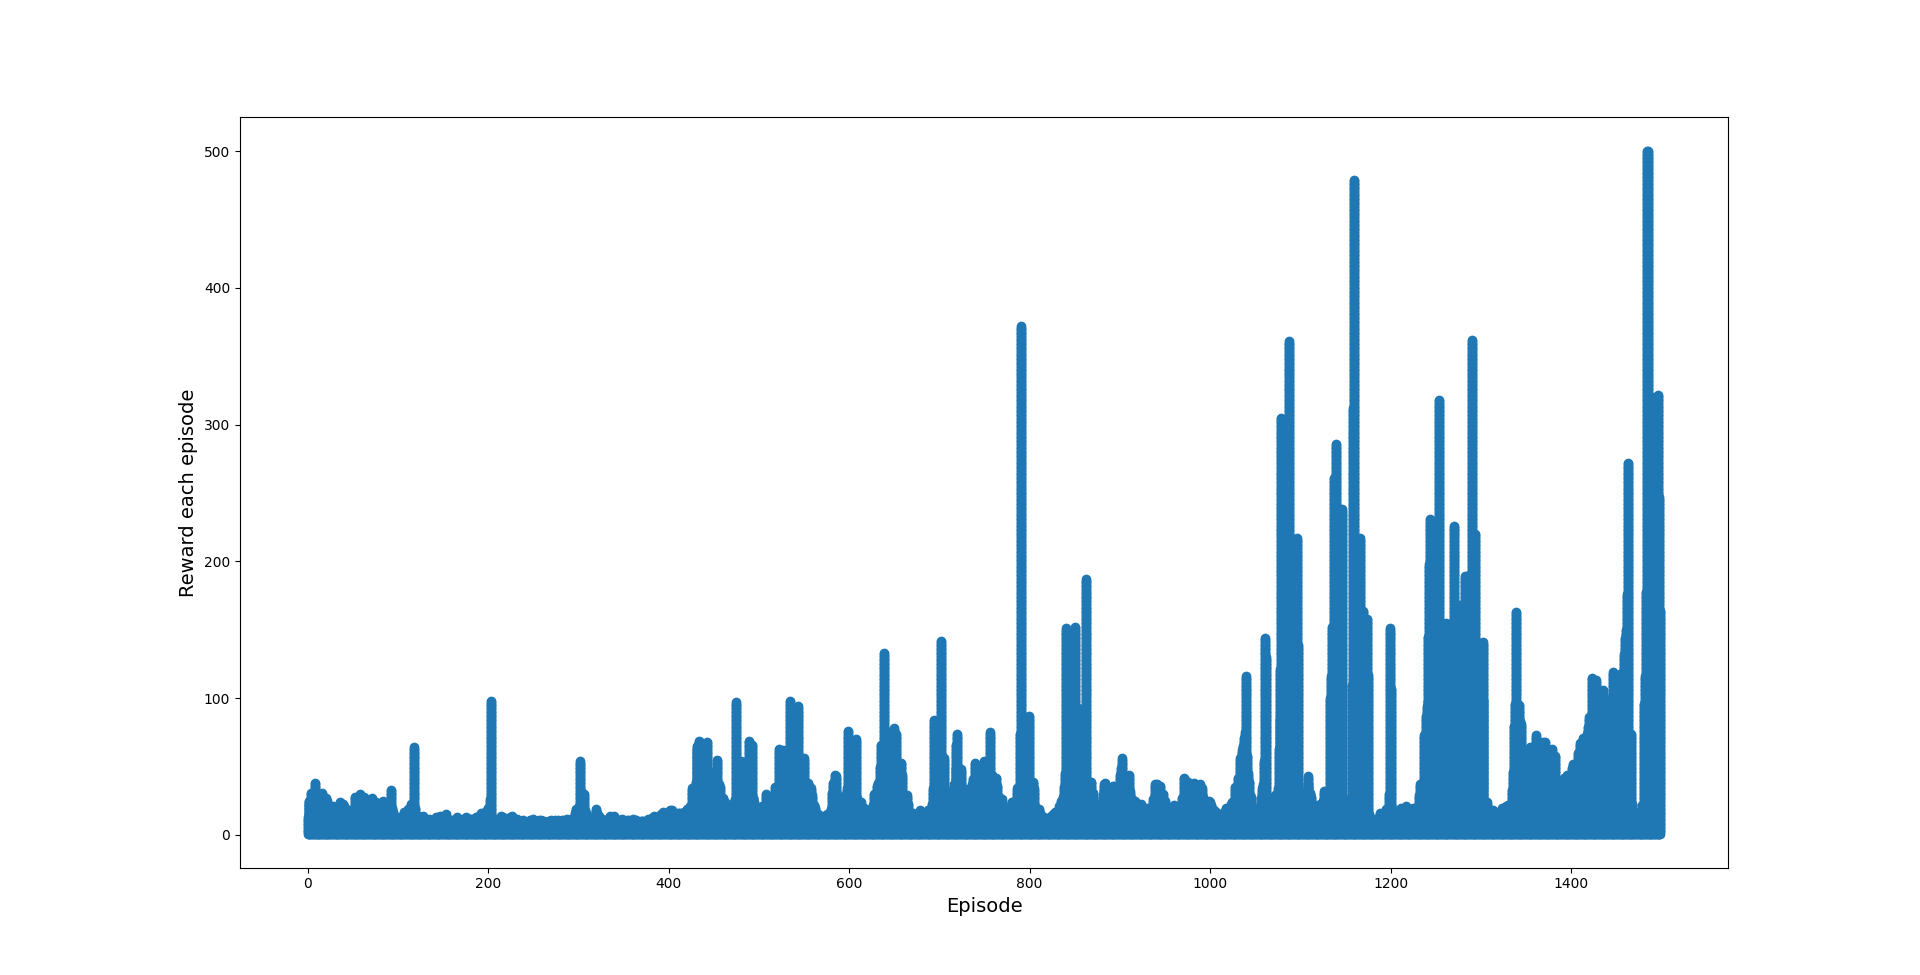
\includegraphics[width=\textwidth,height=\textheight,keepaspectratio]{figures/dqn.png}

We train the model with 1500 episodes. The result is inconsistent. After 200 episodes, the reward exceeds over 100 for the first time, but is very low for the most episodes. As later into training, the reward keep getting better but still very low most of the time.

\subsection{Deep Q-Learning With Experience Replay}

As the task sheet recommend, we add an experience replay buffer to improve the model. The buffer has the size of 10000, and each time we train the model, we sample 128 tuples. The hyper-parameters of the model is the same as the one in the last section.

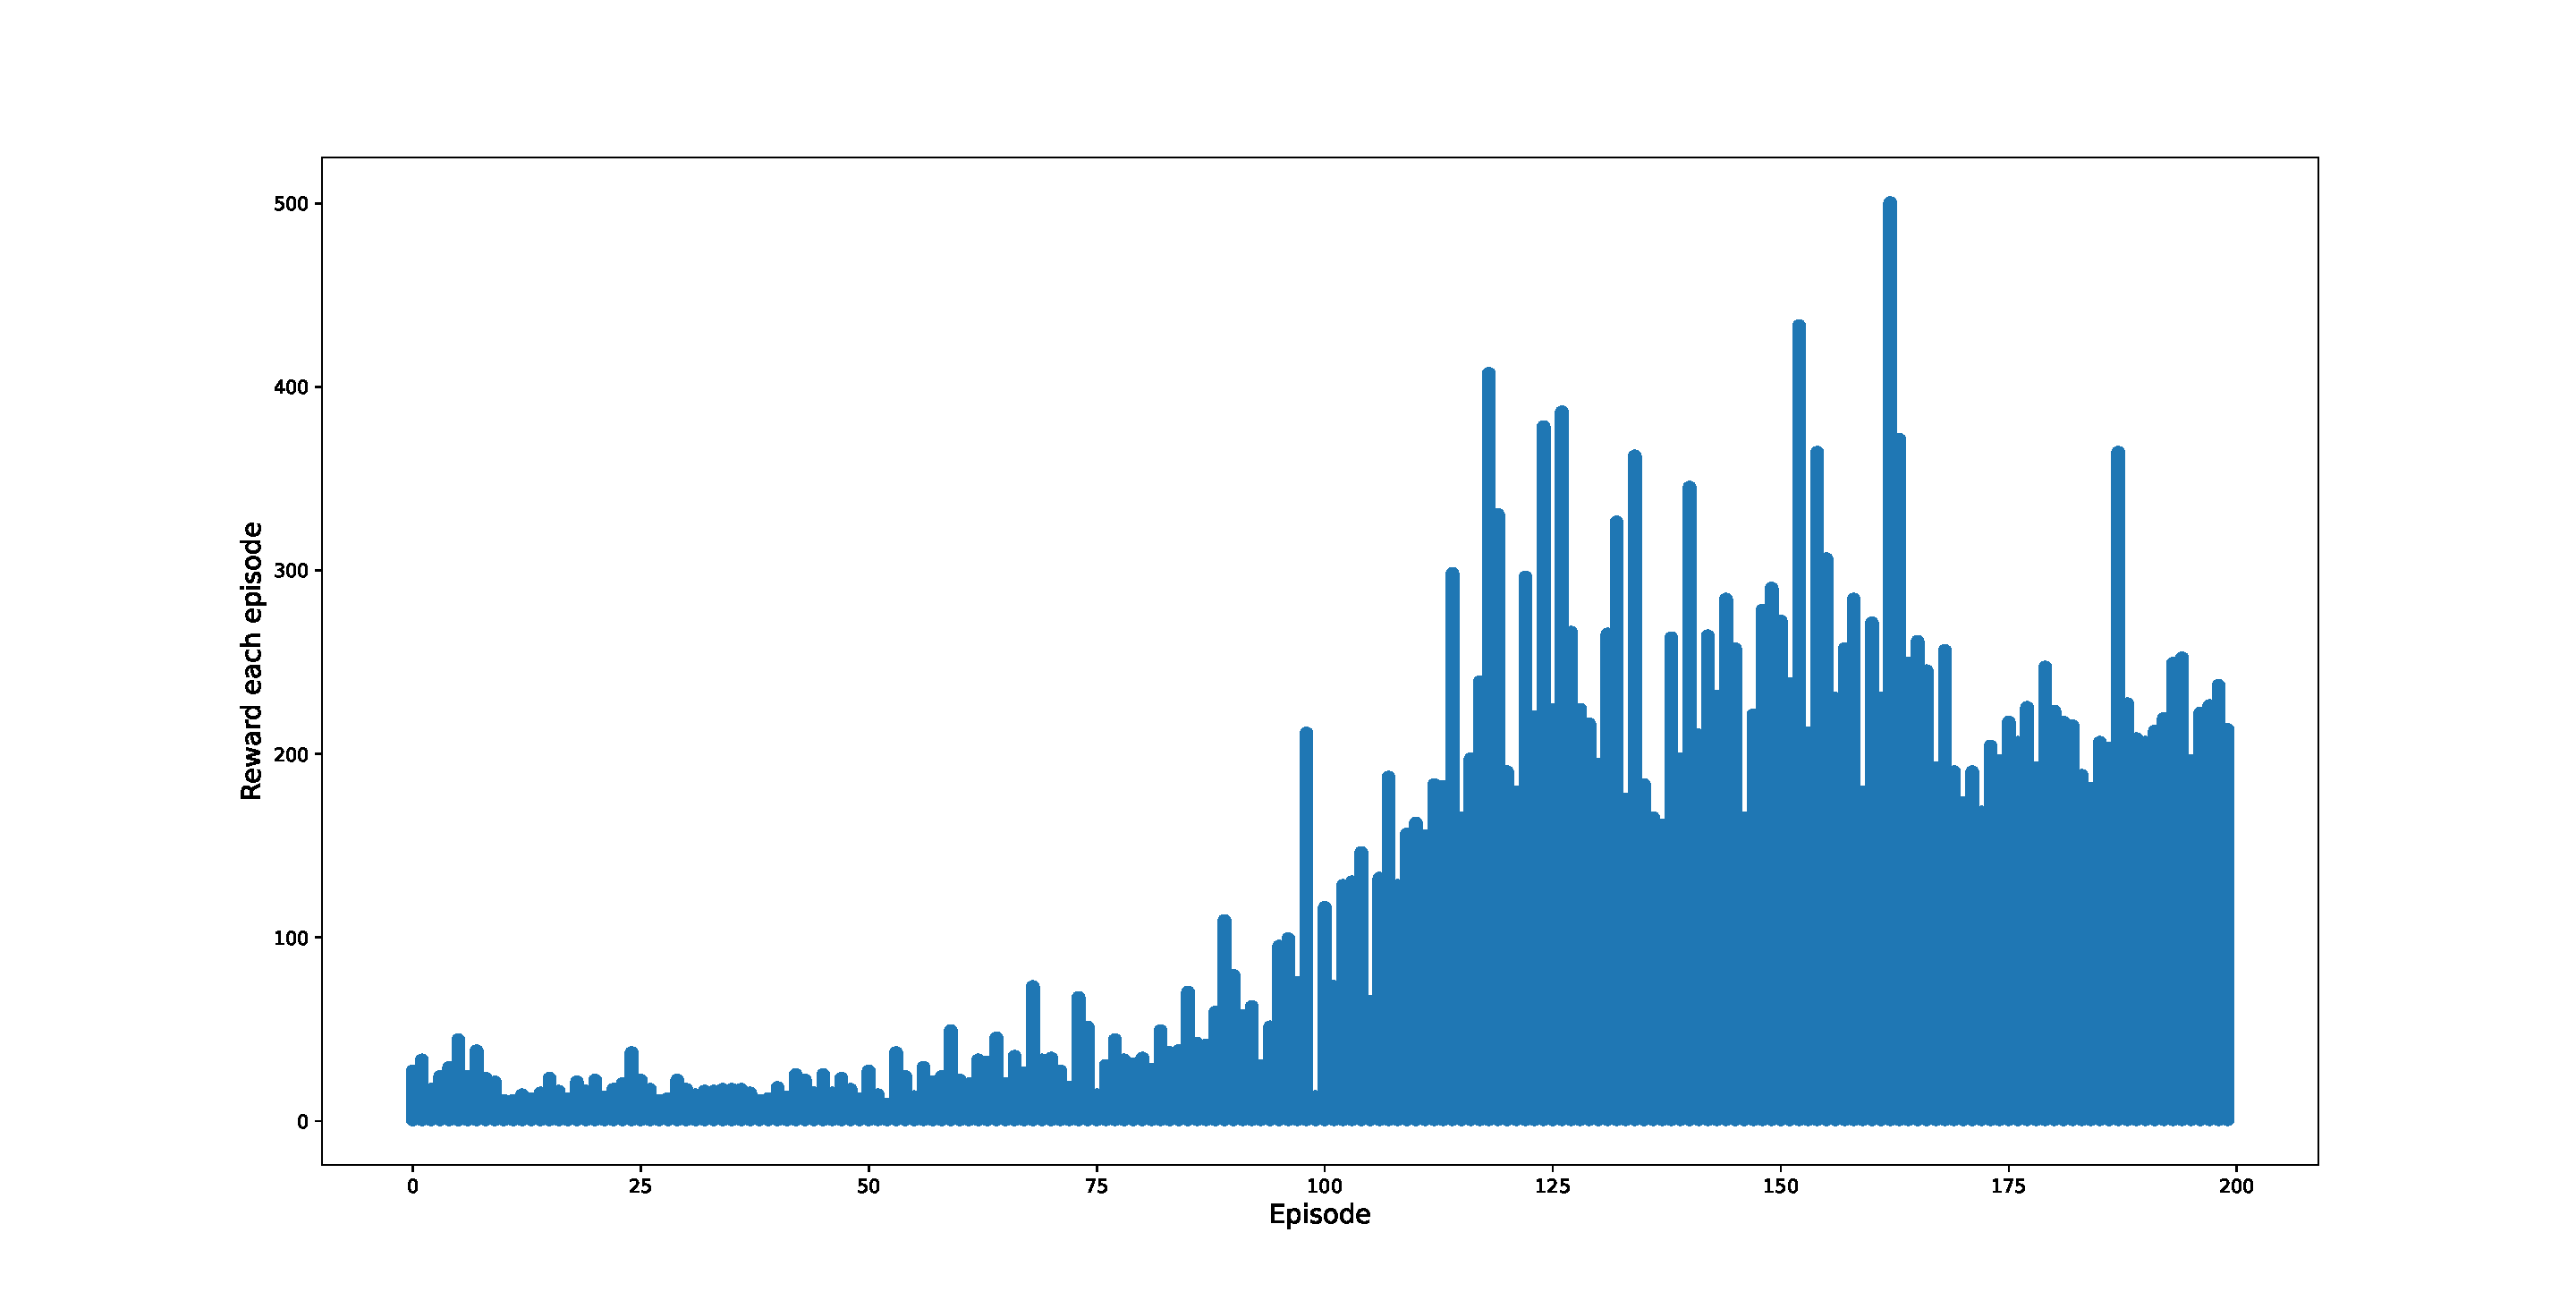
\includegraphics[width=\textwidth,height=\textheight,keepaspectratio]{figures/dqn_buffer.pdf}

The result shown a significant improvement. We only use 200 episodes and the reward exceeds 100 consistently after less than 100 episodes. The peak reward also grow faster compare to the previous approach without a buffer.


% Print references
\end{document}
